Although computer graphics is a vast field that encompasses almost any graphical aspect, we are mainly 
interested in the generation of images of 3-dimensional scenes. Computer imagery has applications for film 
special effects, simulation, training, games, medical imagery, flying logos, etc.

Computer  graphics  relies  on  an  internal \textbf{model} (modeling) of  the  scene, that  is,  a  mathematical representation suitable  for  graphical  computations. The  model  describes  the  3D:

\begin{itemize}
\item shapes
\item layout
\item materials
\end{itemize} 

This 3D representation then has to be projected to compute a 2D image from a given viewpoint, this is 
the \textbf{rendering} step.  Rendering  involves:

\begin{itemize}
\item projecting  the  objects  (perspective)
\item handling visibility (which parts of objects are hidden)
\item computing their appearance and lighting interactions
\end{itemize} 

Finally, for animated sequence, the motion of objects has to be specified. We will not discuss \textbf{animation} in this document.  

\subsection{Modeling}

We introduce how the geometry of the scene is represented in the memory of the computer. 

The most classical method for modeling 3D geometry is the use of polygons. An object is approximated by a \textbf{polygonal mesh}, that is a set of connected polygons. Most of the time, triangles are used for simplicity and generality.

Each polygon or triangle can be described by the 3D coordinates of its list of vertices. The  obvious limitation  of  triangles  is  that  they  produce  a  flat  and  geometric  appearance.  However,  techniques called 	textbf{smoothing  or interpolation} can greatly improve this.

The most classical geometric entities can be directly used as primitives, e.g. cubes, cylinders, spheres and 
cones. A sphere for example can be simply described by the coordinates of its center and its radius.

More  complex  mathematical  entities  permit  the  representation  of  complex  smooth  objects.  \textbf{Spline patches  and  NURBS}  are  the  most  popular. They  are  however  harder  to  manipulate  since  one  does  not directly  control  the  surface  but  so  called control points that are only indirectly related to the final shape. Moreover, obtaining smooth junctions between different patches can be problematic. However, the recently popular subdivision surfaces overcome this limitation. They offer the best of both worlds and provide the simplicity of polygons and the smoothness of patches.

\subsection{Rendering}

The image projection of the 3D objects is computed using linear perspective. Given the position of the viewpoint  and  some  camera  parameters  (e.g.  field  of  view),  it  is  very  easy  to  compute  the  projection of a 3D point onto the 2D image. For mathematics enthusiasts, this can be simply expressed 
using a 4*4 matrix. 

In most methods, the geometric entities are then \textbf{rasterized}. It consists in drawing all the pixels covered by the entity. In the example below, the projections of the 3 red points have been computed using linear perspective, and  the  triangle  has  then  been  rasterized  by  filling  the  pixels  in  black. 

\begin{figure}[H]
\centering
\makebox[\textwidth][c]{
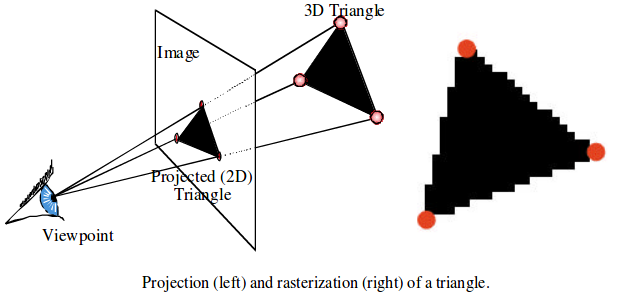
\includegraphics[scale=0.75]{./images/raster.png}
}
\end{figure}

For  richer  rendering,  the  color  of  each rasterized pixel must take into account the optical properties of the object, as we will discuss below. 

\subsubsection{Visibility}

If the scene contains more than one object, \textbf{occlusions} may occur. That is, some objects may be hidden by others. Only visible objects should be represented. Visibility techniques deal with this issue. One classical algorithm that solves the visibility problem is the so-called \textbf{painter's algorithm}.

It consists in  sorting  the  objects  or  polygons  from  back  to  front  and  rasterizing  them  in  this  order.  This  way,  front-most polygons cover the more distant polygons that they hide. 

\begin{figure}[H]
\centering
\makebox[\textwidth][c]{
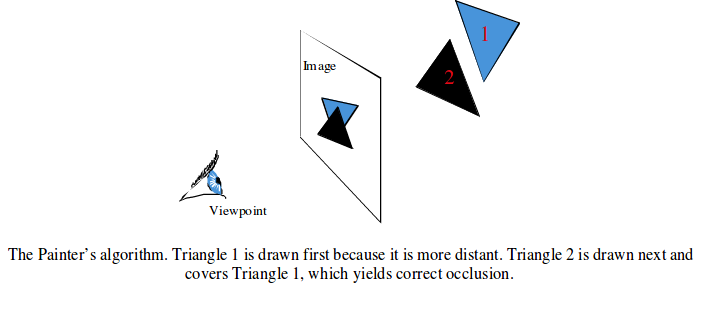
\includegraphics[scale=0.75]{./images/painter.png}
}
\end{figure}

The \textbf{ray-tracing} algorithm does not use a rasterization phase. It sends one ray from the eye and through each pixel of the image. The intersection between this ray and the objects of the scene is computed, and only the closest intersection is considered.

\begin{figure}[H]
\centering
\makebox[\textwidth][c]{
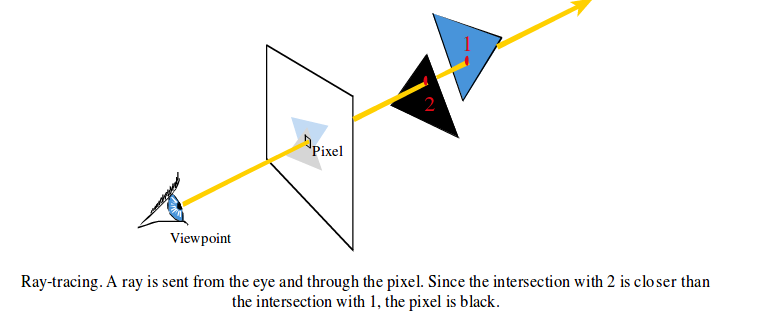
\includegraphics[scale=0.75]{./images/raytrace.png}
}
\end{figure}

The \textbf{z-buffer method} is the most common nowadays (e.g. for computer graphics cards). It stores the depth (z) of each pixel. When a new polygon is rasterized, for each pixel, the algorithm compares the depth of the current polygon and the depth of the pixel. If the new polygon has a closer depth, the color and depth of the pixel  are  updated.  Otherwise,  it  means  that  for  this  pixel,  a  formerly  drawn  polygon  hides  the  current polygon.

\subsubsection{Shading and materials}

Augmenting  the  scene  with  light  sources  allows  for  better  rendering.  The  objects  can  be  
shaded according to their interaction with light. Various \textbf{shading models} have been proposed in the literature. They describe how light is reflected by object, depending on the relative orientation of the surface, light source and viewpoint.

Texture  mapping uses  2D  images  that  are  mapped  on  the  3D  models  to  improve  their  appearance.

Shading and material models only take into account the local interaction of surfaces and light. They do 
not simulate shadows that  are  harder  to  handle  because  they  imply  long-range interactions. A shadow is caused by the occlusion of light by one object. \textbf{Ray-tracing},  for  example,  can  handle  shadows,  but  requires  a  shadow  computation  for  each  pixel  and  each  light  source.  A  shadow ray is sent from the visible point to the light source. If the ray intersects an object, then the visible point is in shadow.

\begin{figure}[H]
\centering
\makebox[\textwidth][c]{
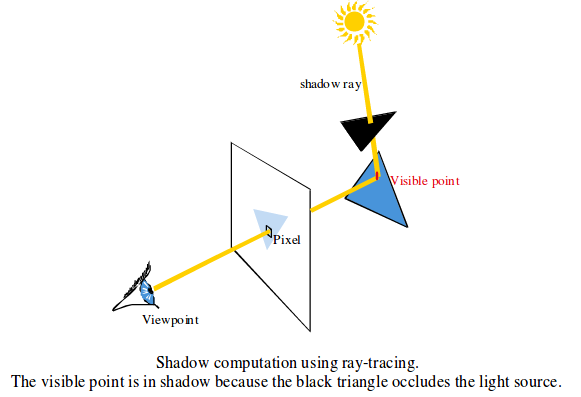
\includegraphics[scale=0.75]{./images/shadow.png}
}
\end{figure}  

More complex lighting interactions can then be \textbf{simulated}. In particular, objects that are illuminated by a primary light  source  reflect  light  and  produce indirect  lighting.  This  is  particularly  important  for  indoor scenes. Global lighting methods take into account all light inter-reflections within the scene.

Rendering can be classified in three categories:

\begin{itemize}
\item \textbf{Non-photorealistic}: rendering of scenes in an artistic style, intended to look like a painting or drawing.
\item \textbf{Photorealistic}: rendering of scenes intended to look like indistinguishable from a photo.
\item \textbf{Physically based}: rendering in a way that more accurately models the flow of light in the real world. 
\end{itemize}

See: \url{http://people.csail.mit.edu/fredo/Depiction/1_Introduction/reviewGraphics.pdf}

\subsection{Exercises}

\begin{exercise}
What of the following matrices corresponds to the 2D transformation: translation of an homogeneous vector $(-1,1,1)$ followed by a rotation of angle $\theta = 270^{o}$.
\end{exercise}
\begin{itemize}
\item We have to multiply matrices $((0,-1,0),(1,0,0),(0,0,1))$ and $((0,-1,1),(1,0,2),(0,0,1))$.
\item The answer is $((0,-1,1),(1,0,2),(0,0,1))$.
\end{itemize}


\begin{exercise}
What of the following equivalences between points in homogeneous coordinates are true?
\end{exercise}
\begin{itemize}
\item $(-1,-1,-1) \sim (1,1,1)$ true, take $\lambda = -1$.
\item $(-1,1,1) \sim (1,-1,1)$ false, no $\lambda$ possible.
\item $(-2,2,-1) \sim (1,-1,1)$ false, no $\lambda$ possible.
\item $(-1,1,0) \sim (1,-1,0)$ true, take $\lambda = -1$.
\end{itemize}




